\section{Introduction}
\label{sec:intro}

\begin{figure}[ht]
    \centering
    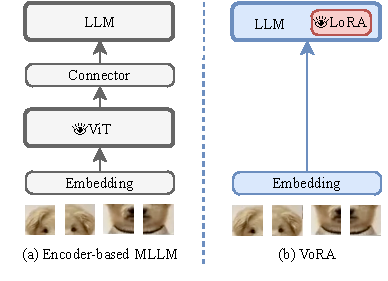
\includegraphics[width=\linewidth]{images/Figure1.pdf}
    \caption{A high-level overview of \model{}. Visual parameters are indicated with an eye icon. Mainstream MLLMs adopt a modular, sequential architecture: raw pixels are first processed by a pre-trained vision encoder to extract high-level visual features, which are then aligned with the LLM through a modality connector for vision-language tasks. In contrast, \model{} consists solely of an LLM and a lightweight embedding layer. The LoRA layers serve as visual parameters that can be integrated into the LLM without incurring additional computational costs or memory burdens. }
    \label{fig:figure1}
\end{figure}

Multimodal Large Language Models (MLLMs) \cite{blip2, llava, llava1_5, flamingo, minigpt} have advanced significantly by integrating pre-trained vision models with Large Language Models (LLMs) \cite{intern1.5, llama, vicuna, gpt3, qwen} through a modular design: visual features extracted by vision encoders to be aligned with LLMs via a connector, as shown in Figure \ref{fig:figure1}(a). While efficient in training, this approach has key limitations derived from the external vision expert models, i.e., extra computational costs and image resolution constraints. For instance, many vision encoders, particularly Vision Transformers (ViTs) \cite{siglip, clip, vit}, adhere to a fixed-resolution training paradigm, limiting flexibility. Additionally, the modular design imposes a sequential workflow: the LLM cannot begin processing until the vision encoder and connector have fully processed the image. To overcome these issues, recent studies \cite{fuyu, eve} have explored unified, encoder-free architectures that process raw pixels directly within a single Transformer (i.e., an LLM), eliminating the need of external vision models. However, such methods face challenges from modality conflicts between vision and language, which would lead to new problems, such as unstable training and catastrophic forgetting issues.

Relevant research \cite{evev2, monointernvl} has made attempts to address modality conflicts through parameter decoupling methods.
% increasingly complex architecture designs, which, however, often result in significant memory burden. 
% For example, EVE \cite{eve} chooses to update the whole LLM during its main training stage, however, a instablitty is observed so that they adopt another seperate stage to only train the embedding layers to stablize training. However, the modality conflicts still remain. 
% Prior works \cite{eve2, monointernvl} address modality conflicts through increasingly complex architectural designs, often at the cost of significant memory overhead. 
For example, Mono-InternVL \cite{monointernvl} introduced a Mixture-of-Experts (MoE) framework \cite{moe}, employing separate expert modules for vision and language processing. Taking a step further, EVEv2 \cite{evev2} decoupled all linear and normalization layers in the LLM. While these approaches helped mitigate modality conflicts, they doubled the LLM’s parameters, complicating the architecture and substantially increasing memory overhead.

% Early approaches, such as Fuyu \cite{fuyu}, relied on training models from scratch using mixed image-text datasets. Though effective, this strategy demanded substantial computational resources and did not capitalize on the rapid advancements in pre-trained LLMs). Subsequent methods sought to address these limitations by building upon existing LLMs through fine-tuning on image-text pairs. For example, EVE \cite{eve} introduced a novel architecture that replaced conventional vision encoders with a lightweight transformer block guided by a ViT. However, its successor, EVEv2 \cite{evev2}, completely abandoned this design, opting instead for a more complex vision framework with expanded parameters. Similarly, Mono-InternVL \cite{monointernvl} and EVEv2 adopted a Mixture-of-Experts (MoE) strategy, which discarded the ViT and replicated the LLM parameters to enable selective activation of specialized components during vision tasks. Though this approach reduces computational overhead, it significantly increases memory requirements, complicates model optimization, and compromises the streamlined architecture of the original LLM.
To address these challenges, we propose Vision as LoRA (\model{}), a method of transforming LLMs into encoder-free MLLMs by integrating vision understanding abilities through Low-Rank Adaptation (LoRA) \cite{lora}. 
While we acknowledge that decoupling vision and language parameters is critical, we wish to avoid dependency on parameter expansion in inference. To this end, \model{} applies trainable LoRA layers to LLMs, which encode the new modality, i.e., vision, while preserving the language knowledge of the original LLM by freezing its parameters, as shown in Figure \ref{fig:figure1}(b). Unlike previous approaches \cite{evev2, monointernvl} that retain vision-specific parameters during inference, \model{} merges LoRA layers into the LLM  after training, incurring near-zero additional computational cost or memory overhead.

Furthermore, \model{} leverages pre-trained vision models as teacher models to inject visual priors into the LoRA layers. Specifically, we adopt the strategy of block-wise distillation \cite{distillation}: the intermediate visual representations of each LLM block are forced to align with the corresponding block-level features extracted by the teacher model. With such a process, we can greatly accelerate training and reduce the demand for massive data. 

In addition, we replace the LLM's causal attention mask with a bi-directional one for image processing, which better captures contextual relations. Meanwhile, we have also found that, unlike most conventional encoder-based MLLMs \cite{qwen, llava, llava1_5, llavaov, minigpt, minigptv2, cogvlm} which are constrained by fixed-resolution vision encoders, \model{} naturally supports native image resolutions by exploiting the LLM’s inherent ability to process variable-length sequences. 
%Through extensive ablation studies and experiments, we validate the effectiveness of each component in \model{} and demonstrate its potential as a robust architecture for the next generation of MLLMs.

Our contributions are threefold: 
\begin{itemize}
    \item \textbf{Framework innovation:} \model{} converts LLMs into MLLMs via: (1) vision as LoRA, (2) block-wise distillation, and (3) bi-directional attention for vision. Parameter decoupling between vision and language pathways stabilizes training, while other components accelerate training and reduce data needs. Ablation studies confirm the effectiveness of each element, establishing \model{} as a new paradigm for encoder-free MLLMs.

    \item \textbf{Performance validation:} When trained with a proper scale of additional data, \model{} matches conventional encoder-based MLLMs in terms of performance while reducing computational costs, demonstrating that LLMs can acquire native multimodal capabilities without external vision models. This challenges the widely perceived necessity of encoder-based architectures for multimodal tasks. 

    \item \textbf{Potential extensibility:} Although we narrow down our scope to vision understanding tasks in this paper, the modality-agnostic architecture of \model{} has the potential of generalizing to other modalities (e.g., audio and point clouds) and tasks (e.g., image generation).
\end{itemize}

% First, \model{} demonstrates a novel paradigm to convert LLMs into MLLMs via three components—LoRA for vision, block-wise distillation, and bidirectional masks. Second, we prove that \mono{} trained with targeted data can rival modular MLLMs in performance. Third, our approach offers broader implications for multimodal systems, from image generation to video understanding, by showing how parameter-efficient adaptation can harmonize modalities without architectural bloat. This work redefines the potential of unified architectures, paving the way for scalable, general-purpose multimodal AI.